\section{Estimation} \label{sec:estimation}

We estimate expected performance of each benchmark on a given database
configuration for the second phase of our solution. In doing so, we
hope to approximately estimate the performance of the target workload
through the estimation for the benchmark it maps to. As such, we train
two estimators for each benchmark: one for database throughput and one
for database latency.

\begin{figure*}
    \centering
    \fbox{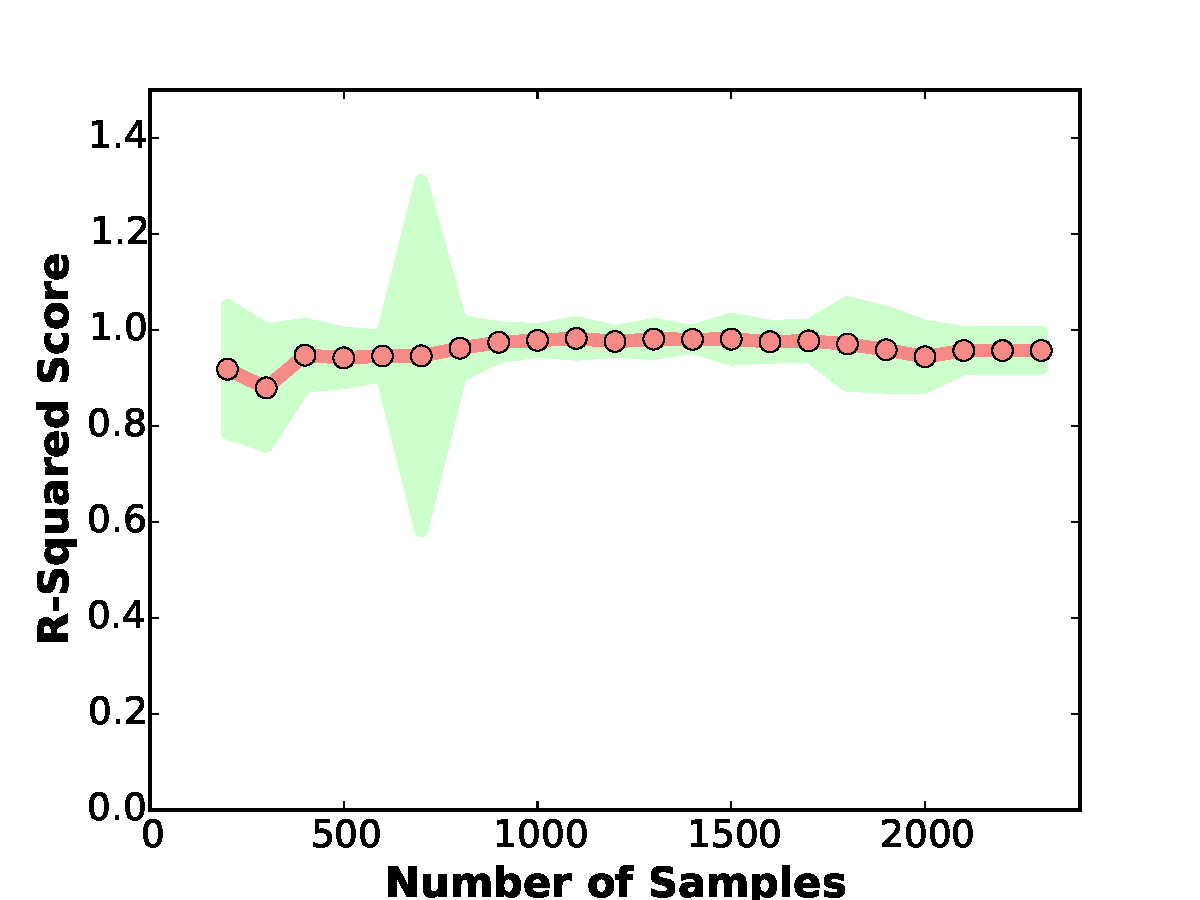
\includegraphics[width=\linewidth]{figure/gp_per_benchmark_r2_scores_latency_mutate.pdf}}
    \caption{Per-Benchmark Gaussian Processes to Estimate Latency}
    \label{fig:gp_r2_latency}
\end{figure*}

\begin{figure*}
    \centering
    \fbox{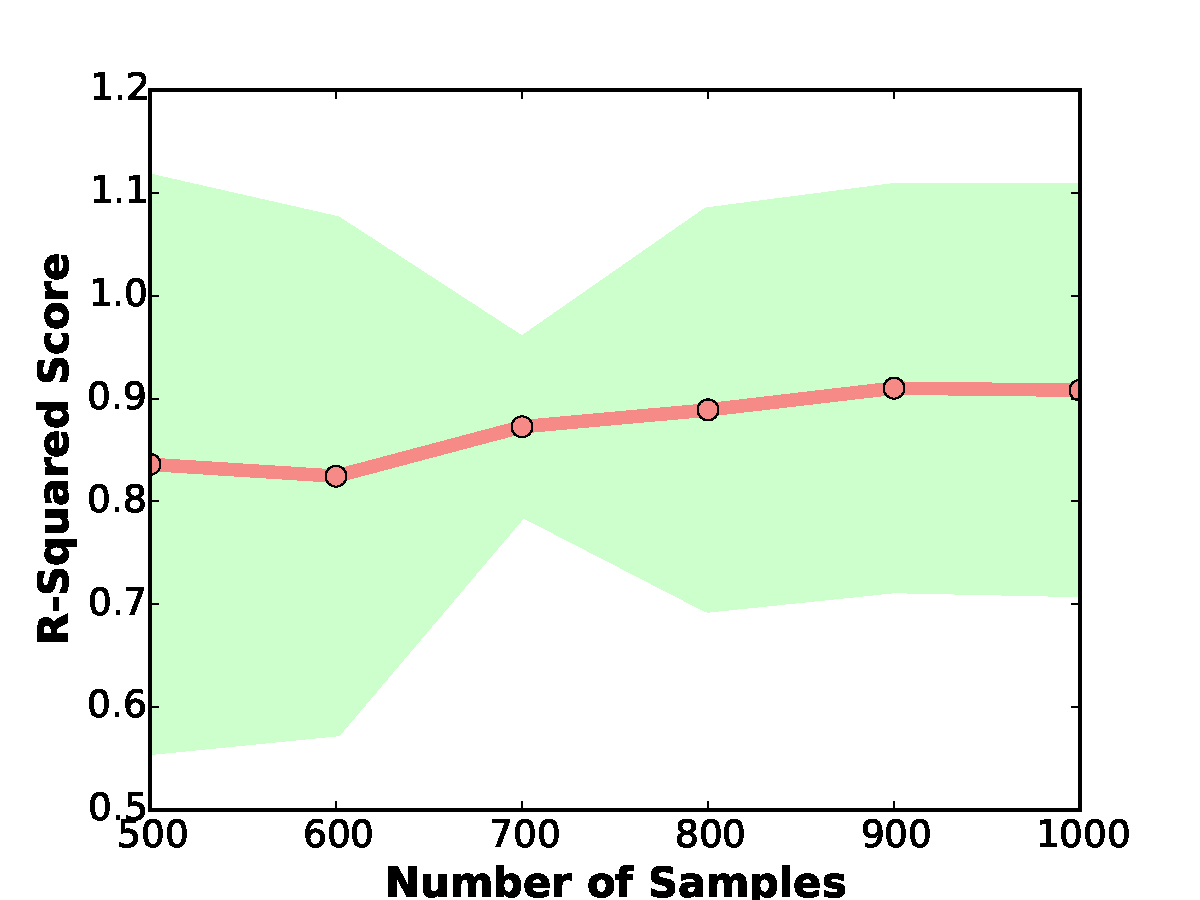
\includegraphics[width=\linewidth]{figure/gp_per_benchmark_r2_scores_throughput_mutate.pdf}}
    \caption{Per-Benchmark Gaussian Processes to Estimate Throughput}
    \label{fig:gp_r2_throughput}
\end{figure*}

We chose to use Gaussian Processes for this task as it works well for
estimating regressions with no prior knowledge about distribution. It
also gives a probabilistic estimation, allowing for further insight
about bounds and probability of exceeding
them. \cref{fig:gp_r2_latency} and \cref{fig:gp_r2_throughput} show
the median $\textrm{R}^2$ score across the estimators for all
benchmarks as a red line. The shaded green region indicates a single
standard deviation spread.

We infer from the figures that we can achieve a very good estimation
with relatively little data. In addition, the the estimators become
better the more data provided, as evidenced by the shrinking green
region as number of samples increases.

\begin{table}
  \centering
  \small{
    \centering
    \begin{tabular}{ll}
      \toprule
      Feature Name                   & Feature Meaning                                                     \\
      \midrule
      AA\_Benchmark                  & Benchmark Name                                                      \\
      PG\_Cache\_Hits                & Number of buffer hits in this table                                 \\
      PG\_Index\_Hits                & Number of buffer hits in all indexes on this table                  \\
      PG\_disk\_blocks\_cache\_hit   & Number of times disk blocks were found already in the buffer cache  \\
      PG\_disk\_blocks\_read         & Number of disk blocks read from this sequence                       \\
      PG\_index\_scans               & Number of index scans initiated on this table                       \\
      PG\_rows\_deleted              & Number of rows deleted by queries in this database                  \\
      PG\_rows\_fetched              & Number of rows deleted by queries in this database                  \\
      PG\_rows\_inserted             & Number of rows inserted by queries in this database                 \\
      PG\_rows\_returned             & Number of rows returned by queries in this database                 \\
      PG\_rows\_updated              & Number of rows updated by queries in this database                  \\
      PG\_sequential\_scans          & Number of sequential scans initiated on this table                  \\
      PG\_transactions\_committed    & Number of transactions in this database that have been committed    \\
      PG\_transactions\_rolled\_back & Number of transactions in this database that have been rolled back  \\
      autovacuum                     & Number of times the autovacuum daemon vacuumed this table           \\
      bgwriter\_delay                & The delay between activity rounds for the background writer         \\
      commit\_delay                  & Time delay before a transaction attempts to flush the WAL buffer    \\
      debug\_print\_plan             & Enable printing the execution plan for each executed query          \\
      fsync                          & Enable making sure that updates are physically written to disk      \\
      log\_planner\_stats            & Enable writing performance statistics of the query planner          \\
      shared\_buffers                & Amount of memory the database server uses for shared memory buffers \\
      synchronous\_commit            & Whether transaction commit will wait for WAL records to be flushed  \\
      track\_activities              & Enable the collection of information on the executing commands      \\
      wal\_buffers                   & Amount of shared memory used for WAL data                           \\
      wal\_level                     & Determine how much information is written to the WAL                \\
      wal\_writer\_delay             & Specify the delay between activity rounds for the WAL writer        \\
      \bottomrule
    \end{tabular}
  }
  % \nocaptionrule
  \caption{Influential Features for Throughput Estimation}
  \label{tab:influential_features_for_throughput}
\end{table}

\begin{table}
  \centering
  \small{
    \centering
    \begin{tabular}{ll}
      \toprule
      Feature Name        & Feature Meaning                                                    \\
      \midrule
      AA\_Benchmark        & Benchmark Name                                                     \\
      PG\_index\_scans      & Number of index scans initiated on this table                      \\
      PG\_sequential\_scans & Number of sequential scans initiated on this table                 \\
      fsync               & Enable making sure that updates are physically written to disk     \\
      synchronous\_commit  & Whether transaction commit will wait for WAL records to be flushed \\
      \bottomrule
    \end{tabular}
  }
  % \nocaptionrule
  \caption{Influential Features for Latency Estimation}
  \label{tab:influential_features_for_latency}
\end{table}

To gain more insight about what parameters affected performance the
most, we performed Lasso Regression to determine the most influential
features. These features are summarized in
\cref{tab:influential_features_for_throughput} and
\cref{tab:influential_features_for_latency}.
